%%%%%%%%%%%%%%%%%%%%%%%%%%%%%%%%%%%%%%%%%
% Beamer Presentation
% LaTeX Template
% Version 1.0 (10/11/12)
%
% This template has been downloaded from:
% http://www.LaTeXTemplates.com
%
% License:
% CC BY-NC-SA 3.0 (http://creativecommons.org/licenses/by-nc-sa/3.0/)
%
%%%%%%%%%%%%%%%%%%%%%%%%%%%%%%%%%%%%%%%%%

%----------------------------------------------------------------------------------------
%	PACKAGES AND THEMES
%----------------------------------------------------------------------------------------

\documentclass{beamer}

\mode<presentation> {

% The Beamer class comes with a number of default slide themes
% which change the colors and layouts of slides. Below this is a list
% of all the themes, uncomment each in turn to see what they look like.

%\usetheme{default} %6
%\usetheme{AnnArbor}
%\usetheme{Antibes} %6
%\usetheme{Bergen}
%\usetheme{Berkeley}
%\usetheme{Berlin}
%\usetheme{Boadilla} 6
%\usetheme{CambridgeUS}
%\usetheme{Copenhagen}
%\usetheme{Darmstadt} 6
%\usetheme{Dresden}
%\usetheme{Frankfurt}
%\usetheme{Goettingen}
%\usetheme{Hannover}
%\usetheme{Ilmenau}
%\usetheme{JuanLesPins}
%\usetheme{Luebeck}
%\usetheme{Madrid}
%\usetheme{Malmoe}
%\usetheme{Marburg}
%\usetheme{Montpellier}
%\usetheme{PaloAlto}
%\usetheme{Pittsburgh}
%\usetheme{Rochester}
\usetheme{Singapore} % 8
%\usetheme{Szeged}
%\usetheme{Warsaw}

% As well as themes, the Beamer class has a number of color themes
% for any slide theme. Uncomment each of these in turn to see how it
% changes the colors of your current slide theme.

%\usecolortheme{albatross}
%\usecolortheme{beaver}
%\usecolortheme{beetle}
%\usecolortheme{crane}
%\usecolortheme{dolphin}
%\usecolortheme{dove}
%\usecolortheme{fly}
%\usecolortheme{lily}
%\usecolortheme{orchid}
%\usecolortheme{rose}
%\usecolortheme{seagull}
%\usecolortheme{seahorse}
%\usecolortheme{whale}
%\usecolortheme{wolverine}

%\setbeamertemplate{footline} % To remove the footer line in all slides uncomment this line
%\setbeamertemplate{footline}[page number] % To replace the footer line in all slides with a simple slide count uncomment this line

%\setbeamertemplate{navigation symbols}{} % To remove the navigation symbols from the bottom of all slides uncomment this line
}

\usepackage{graphicx} % Allows including images
\usepackage{booktabs} % Allows the use of \toprule, \midrule and \bottomrule in tables

%----------------------------------------------------------------------------------------
%	TITLE PAGE
%----------------------------------------------------------------------------------------

\title[Information Bottleneck Decision Trees]{Information Bottleneck as Regularizer for Decision Trees} % The short title appears at the bottom of every slide, the full title is only on the title page

\author{Niels Warncke} % Your name
\institute[TUB] % Your institution as it will appear on the bottom of every slide, may be shorthand to save space
{
Technische Universität Berlin \\ % Your institution for the title page
\medskip
\textit{niels.warncke@gmail.com} % Your email address
}
\date{\today} % Date, can be changed to a custom date

\begin{document}

\begin{frame}
\titlepage % Print the title page as the first slide
\end{frame}

\begin{frame}
\frametitle{Overview} % Table of contents slide, comment this block out to remove it
\tableofcontents % Throughout your presentation, if you choose to use \section{} and \subsection{} commands, these will automatically be printed on this slide as an overview of your presentation
\end{frame}

%----------------------------------------------------------------------------------------
%	PRESENTATION SLIDES
%----------------------------------------------------------------------------------------
%\include{examples.tex}

\section{Learning Problems} % Sections can be created in order to organize your presentation into discrete blocks, all sections and subsections are automatically printed in the table of contents as an overview of the talk
%------------------------------------------------

\begin{frame}
\frametitle{Learning Problems: Classification and Regression}

\begin{definition}
    Let $\mathbb{X}, \mathbb{Y}$ be random variables with an unknown joint probability distribution $P_{\mathbb{X}, \mathbb{Y}}$, $\mathcal{X}, \mathcal{Y}$ their domain and $X \in \mathbb{X}^N, Y \in \mathbb{Y}^N$ be observed samples. Finding a function $f$ such that $E_{\mathbb{X}, \mathbb{Y}}[J(f(\mathbb{X}), \mathbb{Y})]$ is small is called a classification or regression problem. \footnote{
        This definition can be seen as a special case of the definition by Mitchell, 1997: "A computer program is said to learn from experience $E$ with respect to some class of tasks $T$ and performance measure $P$, if its performance in task $T$. measured by $P$, improves with experience $E$."
    }
\end{definition}

\begin{itemize}
    \item Classification: $|\mathcal{Y}| \in \mathbb{N}$ - the target variable represents a category
    \item Regression: $|\mathcal{Y}| \in \mathbb{R}^{D_y}$ - the target can be any vector
    \item Example: Predict if an image shows a cat, predict the age of a person shown in an image.
\end{itemize}


\end{frame}
\section{Decision Trees}
\begin{frame}
   \frametitle{Decision Trees}
   Decision tree inducers provide an algorithm to solve classification and regression problems.
   \begin{itemize}
      \item  A binary decision tree $T$ splits the data: $s_T(x) = x_{i_T} \leq t_{T}$ unless $T$ is a leaf
      \item If $T$ is a leaf, it predicts $T(x) = c_T$ for some constant $c_T$
      \item If $T$ is not a leaf, it creates two subtrees $T_{left}$ and $T_{right}$, and predicts:
      \[   
      T(x) = 
            \begin{cases}

               T_{left}(x) &\quad\text{if}\:  s_T(x) = \text{TRUE} \\
               T_{right}(x) &\quad\text{if}\:  s_T(x) = \text{FALSE} \\
            \end{cases}
      \]
      \item This defines the capacity of the model
   \end{itemize}
\end{frame}


\begin{frame}
   \frametitle{Decision Trees - Example}
   \begin{center}
      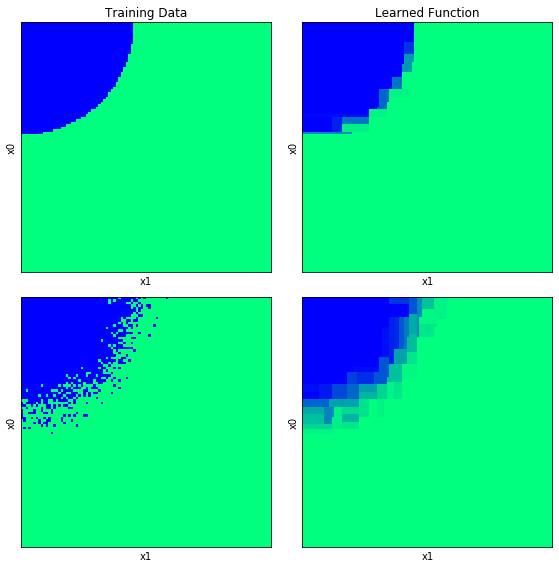
\includegraphics[height=150px]{img/true_vs_learned_regulartree.png}
   \end{center}
   \textit{Left:} Training data of an artificial classification problem. 
   \textit{Right:} Learned function of a decision tree
\end{frame}


\begin{frame}
   \frametitle{Decision Trees - Learning}  
   \begin{itemize}
   \item Fitting a tree is an optimization problem
   \item Many exact solutions are NP hard: e.g. finding a minimal tree that fits the data
   \item Instead of exact solutions: greedy algorithms (bottom up vs top down)
   \item Different loss functions have been proposed: \newline
   InformationGain, Gini Index,  Likelihood-Ratio Chi–Squared Statistics, DKM Criterion, Gain Ratio, ...- see \cite{rokach_decision_2005}
   \item This project evaluates the Information Bottleneck as loss function 
   \end{itemize}
\end{frame}



\begin{frame}[fragile]
   \frametitle{Decision Trees - Top Down}  
   \begin{lstlisting}[language=Python, basicstyle=\small]
class DecisionTree():
  def fit(self, X, Y):
    best_loss = infinity
    for d in range(X.shape[1]): # O(D) 
      loss, thresh, left_split, right_split = \
        best_split(X[:,d], Y) # O(N)
      if loss_d < best_loss:
        update best_loss, X_l, Y_l, X_r, Y_r, t_T, i_T
    if stopping_criterion is fulfilled:
      self.c_T = best_constant_estimator(Y)
      return self
    self.left = DecisionTree().fit(X_l, Y_l)
    self.right = DecisionTree().fit(X_r, Y_r)
    self.prune()
    return self
\end{lstlisting}

Time complexity: $O(N*D*depth(T)) \subseteq O(N*D*log_2(N))$
\end{frame}
\section{Information Bottleneck} % Sections can be created in order to organize your presentation into discrete blocks, all sections and subsections are automatically printed in the table of contents as an overview of the talk
%------------------------------------------------

\begin{frame}
\frametitle{Problem and Algorithm}
Sed iaculis dapibus gravida. Morbi sed tortor erat, nec interdum arcu. Sed id lorem lectus. Quisque viverra augue id sem ornare non aliquam nibh tristique. Aenean in ligula nisl. Nulla sed tellus ipsum. Donec vestibulum ligula non lorem vulputate fermentum accumsan neque mollis.\\~\\

Sed diam enim, sagittis nec condimentum sit amet, ullamcorper sit amet libero. Aliquam vel dui orci, a porta odio. Nullam id suscipit ipsum. Aenean lobortis commodo sem, ut commodo leo gravida vitae. Pellentesque vehicula ante iaculis arcu pretium rutrum eget sit amet purus. Integer ornare nulla quis neque ultrices lobortis. Vestibulum ultrices tincidunt libero, quis commodo erat ullamcorper id.
\end{frame}
\section[Comparison]{Comparison of the Information Bottleneck Iterative Algorithm and Decision Trees} 

\begin{frame}
\frametitle{Comparison: Decision Trees and Information Bottleneck Iterative Algorithm}

- common:
    - find predictive function:
        Trees: X -> leaf -> Y
        IBIA: X -> X' -> Y
    - usage of loss function that can be expressed as expectation
- differences:
    - IB assumes knowledge of $P_{\mathbb{X}, \mathbb{Y}}$
    - IB finds an optimal solution, DT can get stuck in local optima
    - DT is sensitive to the parameterization of $\mathbb{X}$
    - IB requires finite $\mathcal{X}$ or explicit quantization

\end{frame}
\section[IB in Trees]{Information Bottleneck in Decision Trees} % Sections can be created in order to organize your presentation into discrete blocks, all sections and subsections are automatically printed in the table of contents as an overview of the talk
%------------------------------------------------

\begin{frame}
\frametitle{Information Bottleneck in Decision Trees}
- plug in LIB into decision tree inducer
- time and space complexity of the algorithm not affected
- IB now applicable to samples, when PXY unkown
- Generalization bounds?

\end{frame}
\section{Experiments} % Sections can be created in order to organize your presentation into discrete blocks, all sections and subsections are automatically printed in the table of contents as an overview of the talk
%------------------------------------------------

\begin{frame}
\frametitle{Problem and Algorithm}
    - Solutions for different beta
    - For a problem with known distribution: how close are the approximated mutual informations to the real ones
    - for a real world dataset: IB vs basic tree in sklearn

\end{frame}

%------------------------------------------------

\begin{frame}
\frametitle{References}
\footnotesize{
\begin{thebibliography}{99} % Beamer does not support BibTeX so references must be inserted manually as below
\bibitem[Smith, 2012]{p1} John Smith (2012)
\newblock Title of the publication
\newblock \emph{Journal Name} 12(3), 45 -- 678.
\end{thebibliography}
}
\end{frame}

%------------------------------------------------



\begin{frame}
\Huge{\centerline{The End}}
\end{frame}

%----------------------------------------------------------------------------------------

\end{document} 